\chapter{Twitter上の情報を用いた提案認証システム}\label{chap:system}
\section{既存システムの問題点}
既存のライフログを用いた認証方式の問題点として,
\begin{enumerate}
  \item 本人の趣味趣向を真似ることによってなりすましが行いやすい(Web履歴を用いた認証)
  \item GPSのデータを逐一送信できないと認証の安全性が確保できない(GPSを用いた認証)
  \item 重要であったりプライベートなメールが認証時に表示されてしまうことで,情報漏洩やプライバシー情報流出の可能性がある(電子メールを用いた認証)
  \item メッセージ機能を用いて秘密の質問を定期的に更新しているだけで,SNS上でそれを実行する必要性が希薄である(TwitterのDirect Messageを用いた認証)
  \item 友人が自分の顔にのみタグ付けしているという保証がなく(他の動物や物体にも名前のタグ付けが可能),その場合答えられないという状況が発生しうる(友人の顔写真を用いた認証)
\end{enumerate}
などが挙げられる.

\section{採用手法の概要}
前節の問題点するためには,それらを3つに大別した上でそれぞれについて以下のような改善策を用意できると考えた.
\begin{itemize}
  \item 安全性が損なわれる状況が存在する(1,2):特定の趣向や環境に依存しにくい情報を利用する
  \item 認証時に問題が生じる(3,5):ある程度公開されている情報を用いたり,イレギュラーをフィルタリングしやすいように文字情報を主として用いる
  \item 利便性について提案以前の状態から改善できていない(4):能動的に憶えるのではなく,憶えていることを認証に利用する
\end{itemize}
そして提案システムではSNSの情報,今回はTwitter上にある自分のツイートを利用することで上記の改善策を取り入れることができると考えた.
積極的理由として,
\begin{enumerate}
\item 能動的な行為によって生成される情報であり,記憶のための負担に配慮可能なこと
\item 生成された日時の詳細が確実に取得でき,時系列を提示することにより記憶を思い出しやすいこと
\end{enumerate}
が挙げられ,他にも考えうる手段としては以下の様なものがあったが,記載の問題点により前述の手法をとることにした.
\begin{itemize}
  \item 音楽を用いて認証を行う方法
  \begin{itemize}
    \item 外部の騒音などにより認証を行いにくい場面が存在する
    \item 趣味趣向に大きく依存してしまう
  \end{itemize}
  \item Twitterのお気に入り情報を用いる手法
  \begin{itemize}
    \item お気に入りに登録した日時が取得できない
    \item お気に入りに登録したツイートが投稿者により削除される可能性がある
  \end{itemize}
\end{itemize}

また,時系列における情報を保持していることの特徴として,時間情報によって範囲を指定することで,秘密となる情報群を抽出することができるというものがある.
また,相対的な時間情報の指定を行うことで秘密情報の対象を自動で入れ替えることが可能となる.
これによる具体的な利点は\ref{sec:feature}節にて示す.

\section{システムの詳細}
本論文における提案システムとして,前節の内容を踏まえて,利便性(憶えやすさ/使いやすさ)と安全性の両立を目指した個人認証手法を実装した(以下Notifauth).
Notifauth起動時の画面は図\ref{fig:notifauthHome}のようになっており,この画面から新規登録画面(図\ref{fig:notifauthLogin})\footnote{Twitterと連携するためOAuthを用いた}への遷移,設定画面への遷移,実験の試行を開始,実験結果の送信を行うことが可能となっている.

\subsection{秘密情報の設定}\label{subsec:selectSecret}
この手法を用いた秘密の設定方法として,
\begin{description}
  \item[Auto Mode Type Term]\mbox{}\\
    ○日/週/月/年前から△日~年間を指定し,認証時点にその範囲に当てはまるツイートが秘密情報となる(図\ref{fig:notifauthAutoTerm})
  \item[Auto Mode Type Cycle]\mbox{}\\
    ○曜日の△時台という条件に当てはまるツイートが秘密情報となる(図\ref{fig:notifauthAutoCycle})
  \item[Manual Mode]\mbox{}\\
    自分のツイートから任意に1つ秘密情報となるものを選ぶ(図\ref{fig:notifauthManual})
\end{description}
以上の3つを実装した.

\begin{figure}[ht]
  \begin{minipage}{0.5\hsize}
    \begin{center}
      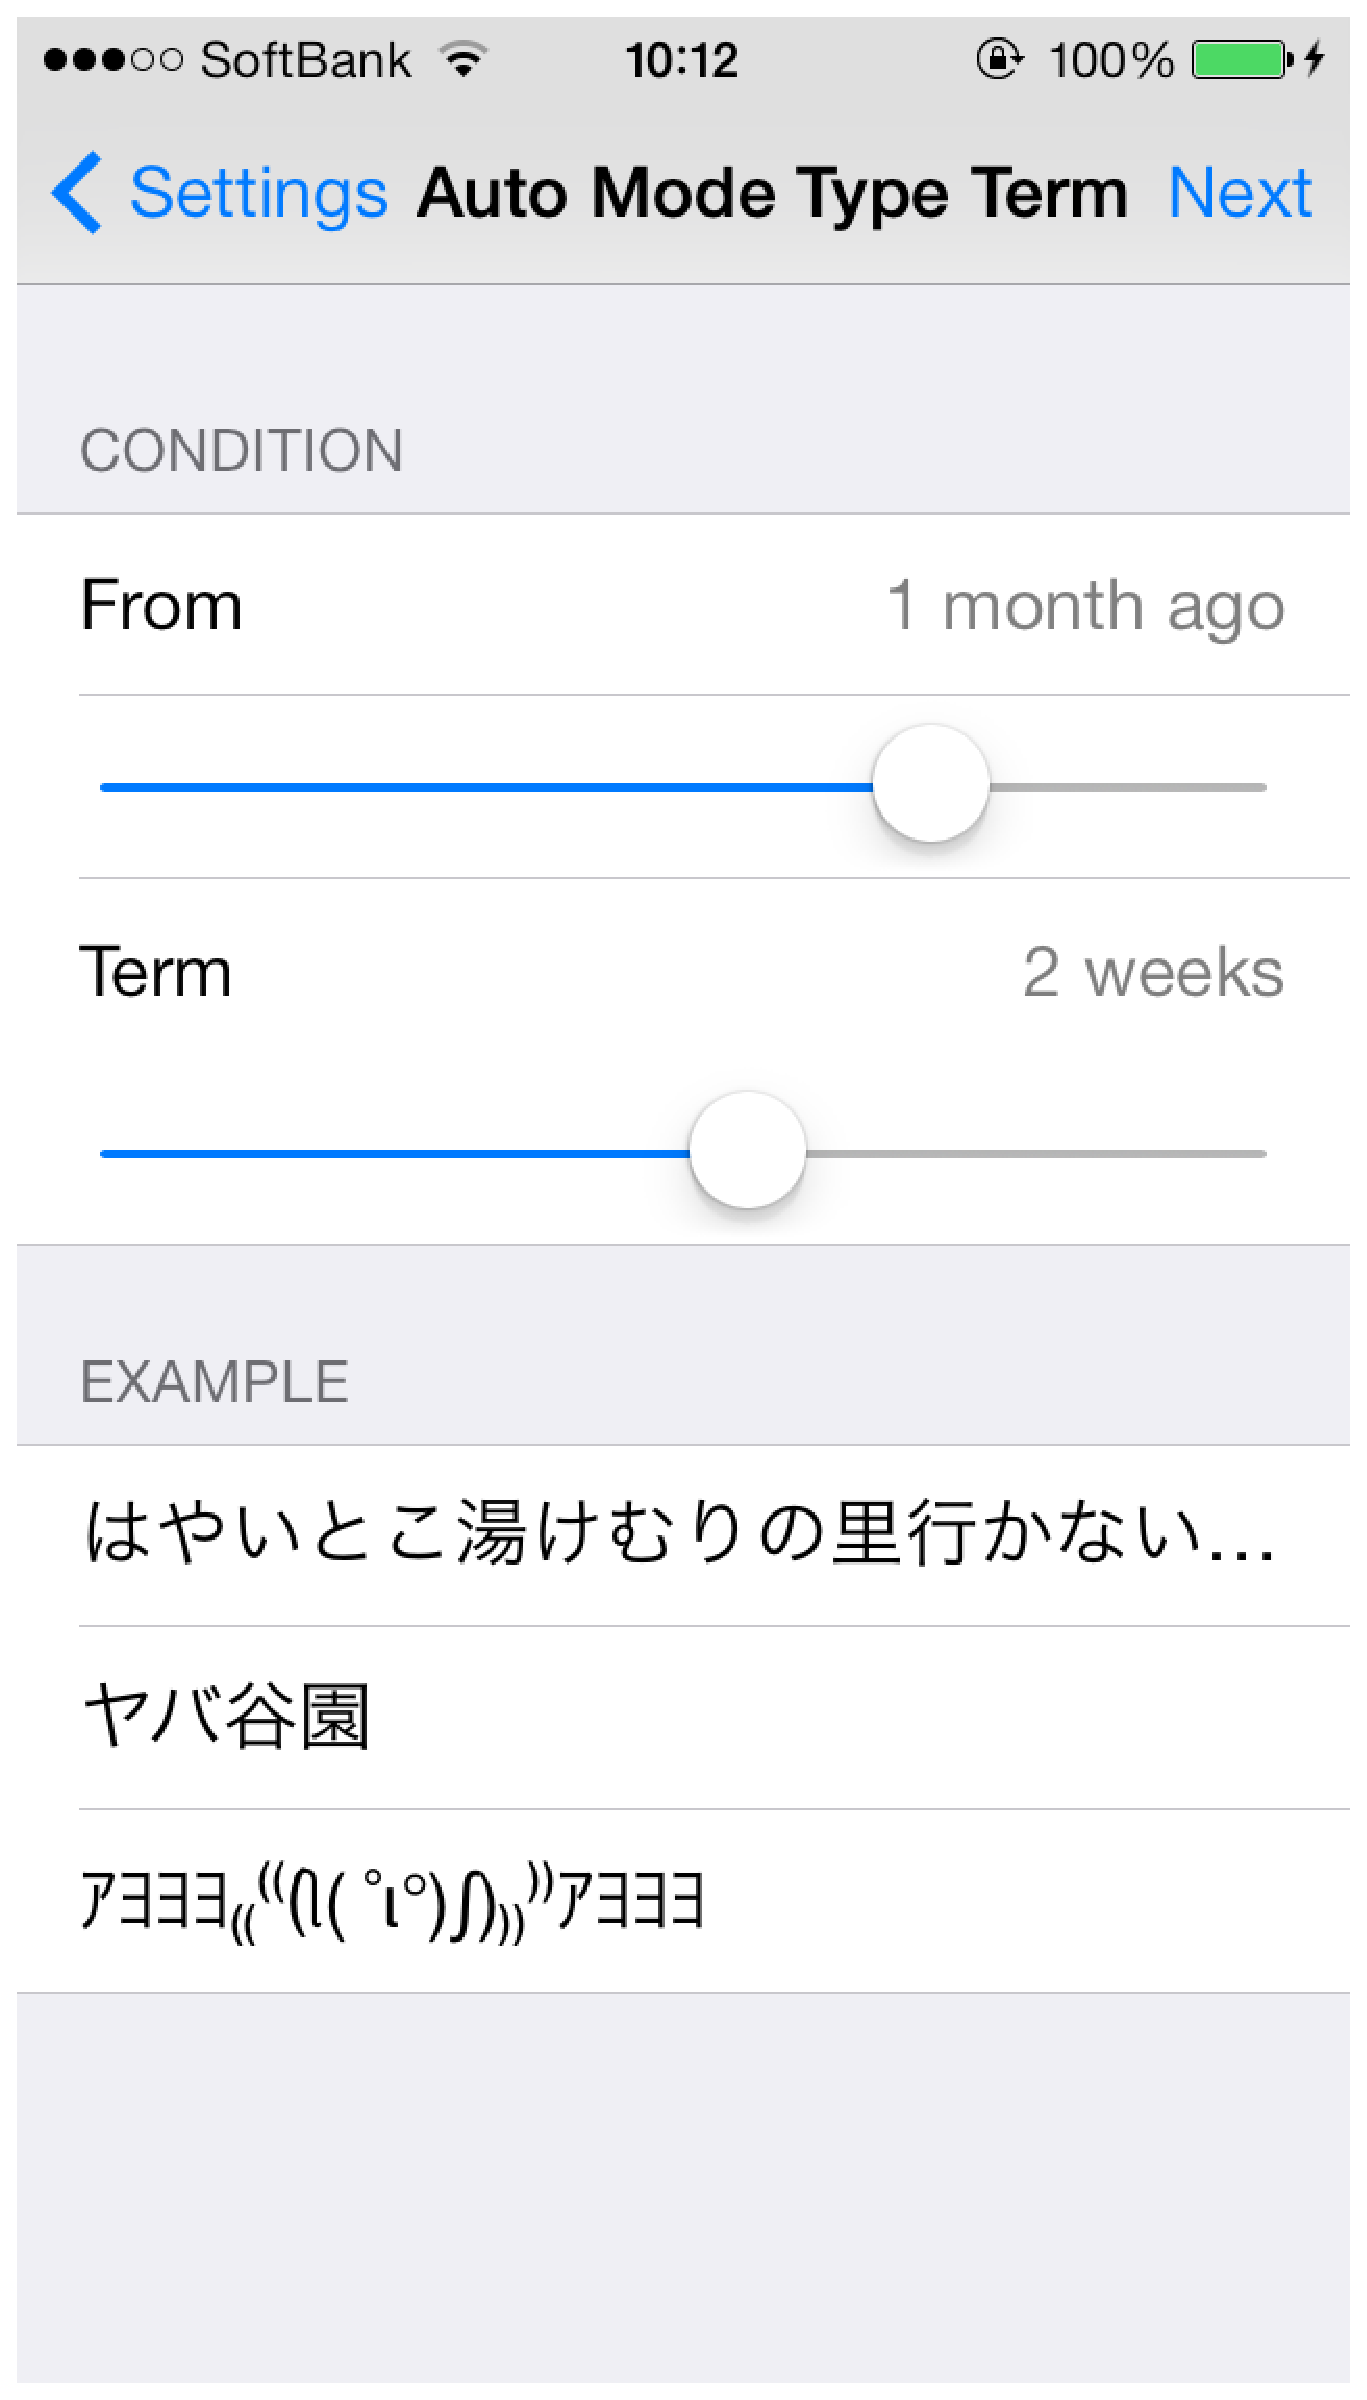
\includegraphics[width=60mm]{img/notifauthAutoTerm.eps}
    \end{center}
    \caption{Auto Mode Type Termの設定画面}
    \label{fig:notifauthAutoTerm}
  \end{minipage}
  \begin{minipage}{0.5\hsize}
    \begin{center}
      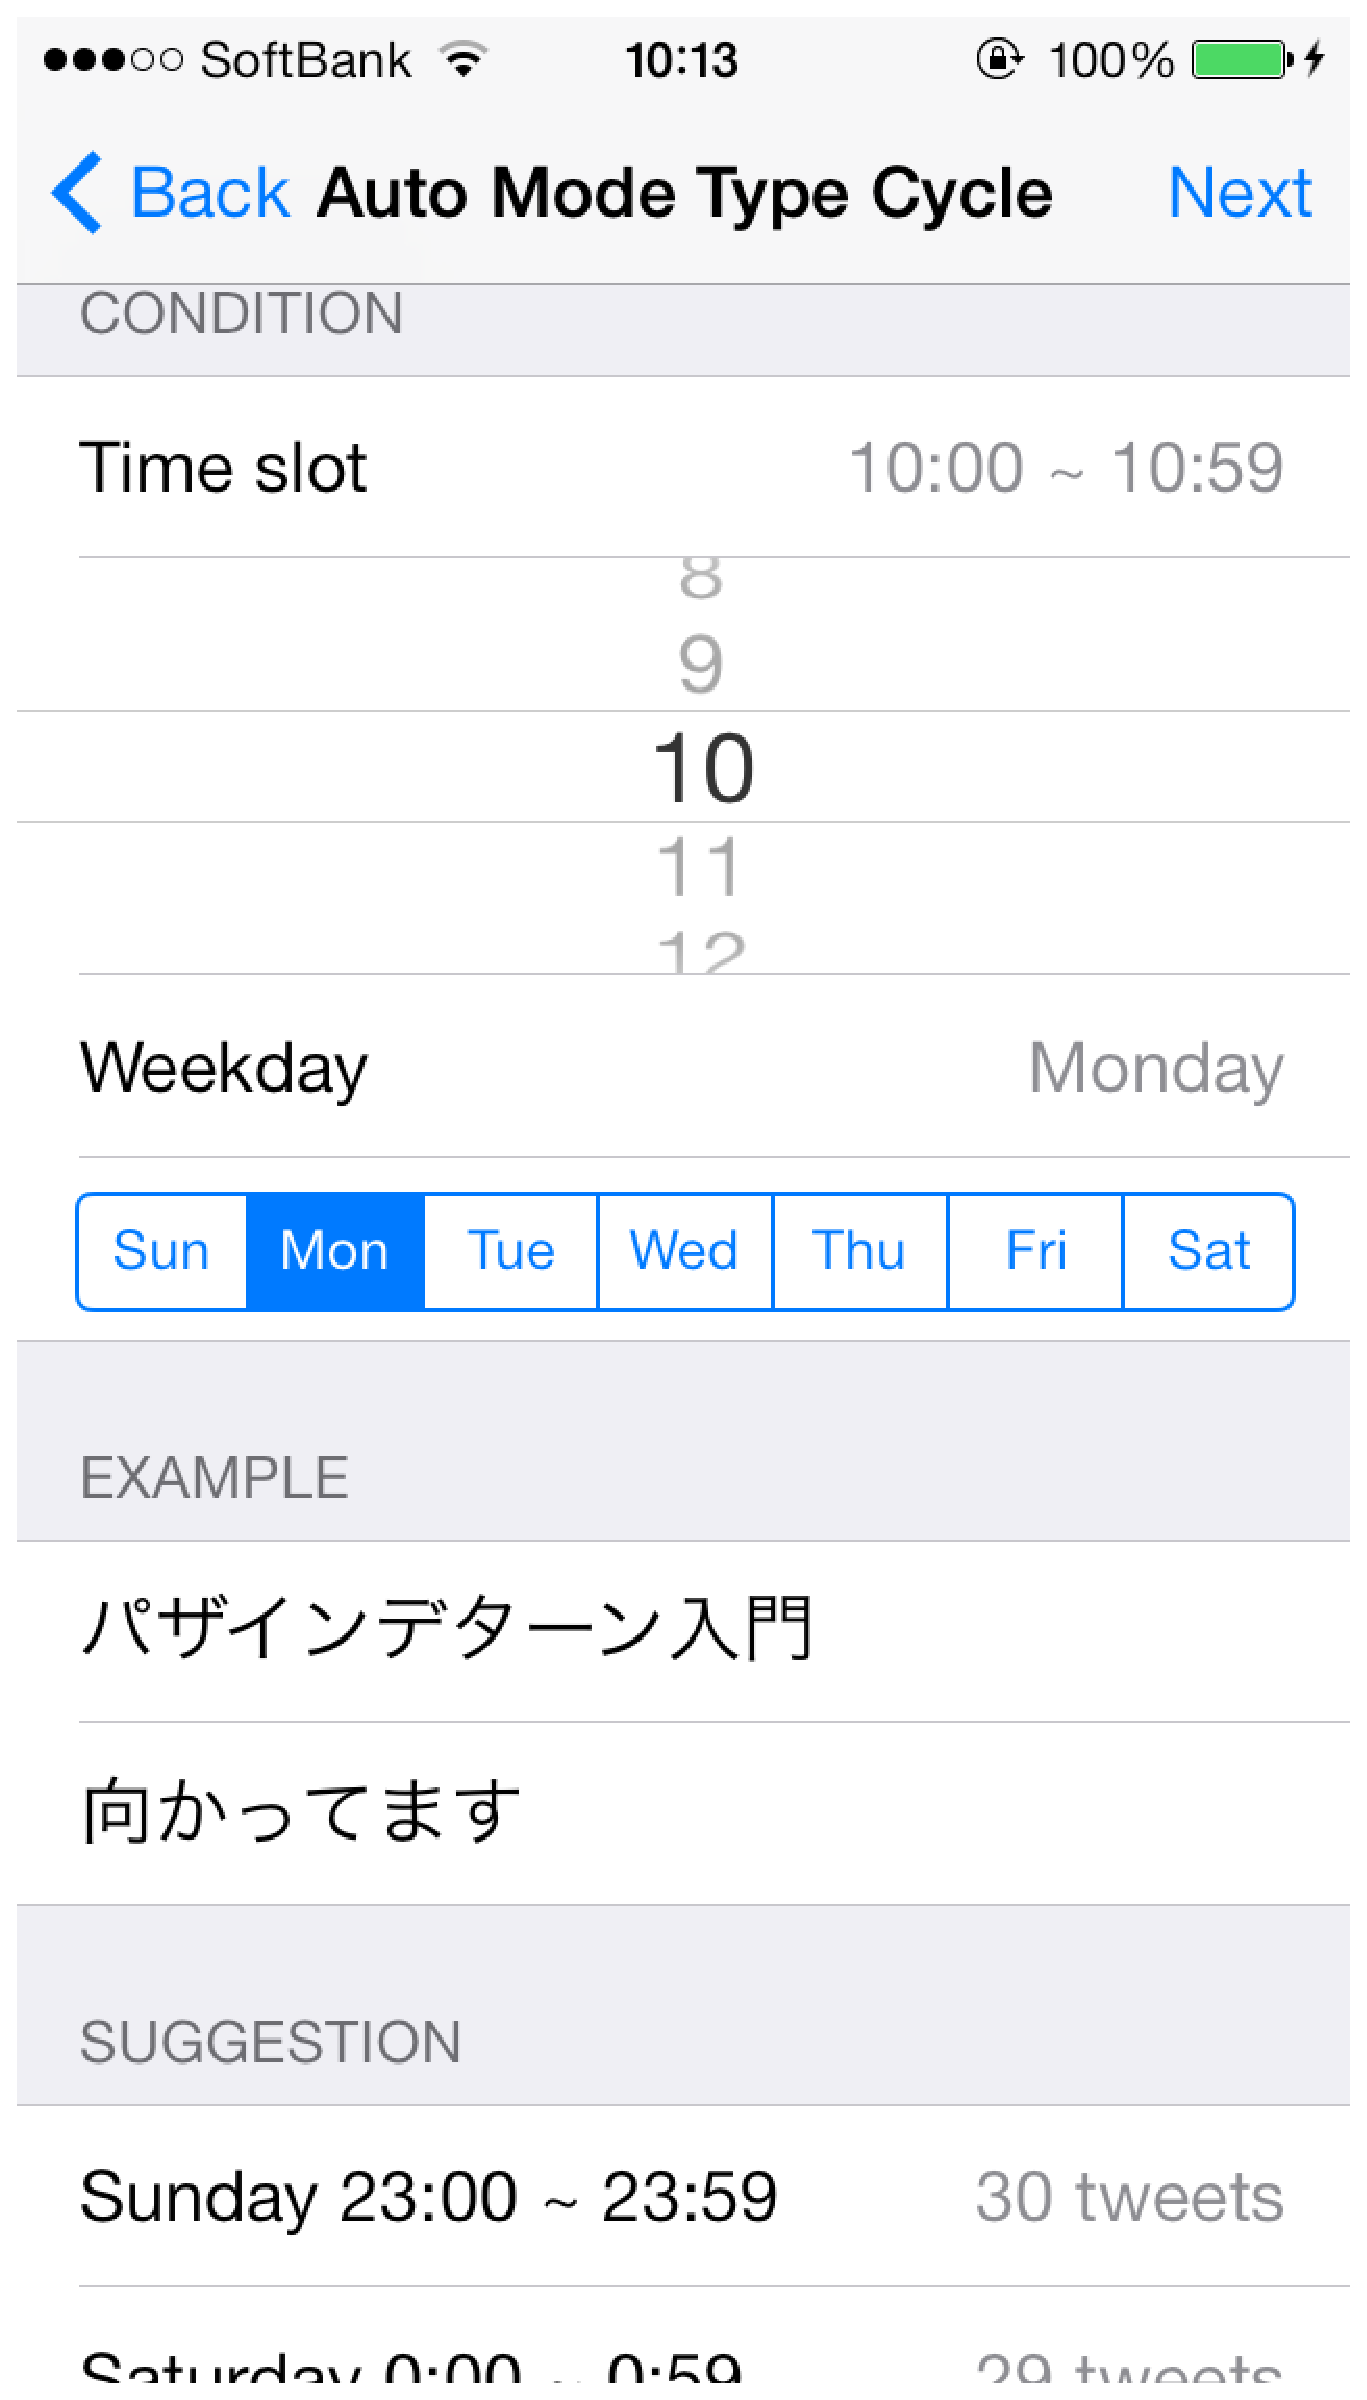
\includegraphics[width=60mm]{img/notifauthAutoCycle.eps}
    \end{center}
    \caption{Auto Mode Type Cycleの設定画面}
    \label{fig:notifauthAutoCycle}
  \end{minipage}
\end{figure}

次に,各設定方法の概要を説明する.

Auto Mode Type Termでは,画面上段の「CONDITION」においてスライダーを用いて「From」(どのくらい前のツイートから秘密情報とするか)と「Term」(Fromからどのくらいの期間のツイートを秘密情報とするか)を設定する.
各スライダーの最大値は,Notifauthによって取得しデータベースに保持されているツイートの中から最も古いものを基準として用いる.
また,画面下段の「EXAMPLE」に,秘密情報として該当するツイートの一部(1行目が最古のもの,3行目が最新のもの,2行目はツイート群の配列の中央値のもの)を表示し,ユーザの設定を補助する.

Auto Mode Type Cycleでは,画面上段の「CONDITION」においてピッカーを用いて「Time slot」(1時間単位で,何時のツイートを秘密情報とするか)を,セレクターを用いて「Weekday」(何曜日のツイートを秘密情報とするか)を設定する.
また,画面中断の「EXAMPLE」に,秘密情報として該当するツイートの一部(1行目が最古のもの,3行目が最新のもの,2行目はツイート群の配列の中央値のもの)を表示し,画面下段の「SUGGESTION」にはNotifauthによって取得しデータベースに保持されているツイートの中で投稿回数が多い曜日・時間の組み合わせを上位3つ表示する.
これらを参考にすることでユーザの設定を補助する.

\begin{figure}
  \begin{center}
    \includegraphics[width=60mm]{img/notifauthManual.eps}
  \end{center}
  \caption{Manual Modeの設定画面}
  \label{fig:notifauthManual}
\end{figure}

Manual Modeでは,直近のツイートを最大200件取得し,これのうちどれを秘密情報とするかを手動で選択し設定する.
ここで設定したツイートは,もう一度設定しない限りは実験終了まで固定されたままである.

\subsection{認証操作}
認証操作としてiOSに実装されているロック画面上の通知とその選択操作(図\ref{fig:notificationSliding}\footnote{この場面ではスライドすることでロック解除後に受信したメールをすぐに読むことができる})を踏襲したものを採用した.
理由として,
\begin{enumerate}
  \item 本システムは携帯端末における認証の多要素化を目指して実装され,その際開発環境であるiOSでそういった操作を行えるのはロック画面のみであったため
  \item ロック画面で通知をスライドし選択する動作はiOS標準の機能であり,ユーザへ新たな操作を覚えさせる負担が少ないと考えたため
\end{enumerate}
が挙げられる.
また,実験を行いやすくするために本論文中の実装では,上記のロック画面を模した環境(図\ref{fig:notifauthNotificationTest},図\ref{fig:notifauthPINTest})をアプリケーション内に実装した.

\begin{figure}[ht]
  \begin{center}
    \epsfig{file=img/notificationSliding.eps,scale=0.35}
  \end{center}
  \caption{ロック画面上における通知の選択(スライド)動作の例}
  \label{fig:notificationSliding}
\end{figure}

\begin{figure}[ht]
  \begin{minipage}{0.5\hsize}
    \begin{center}
      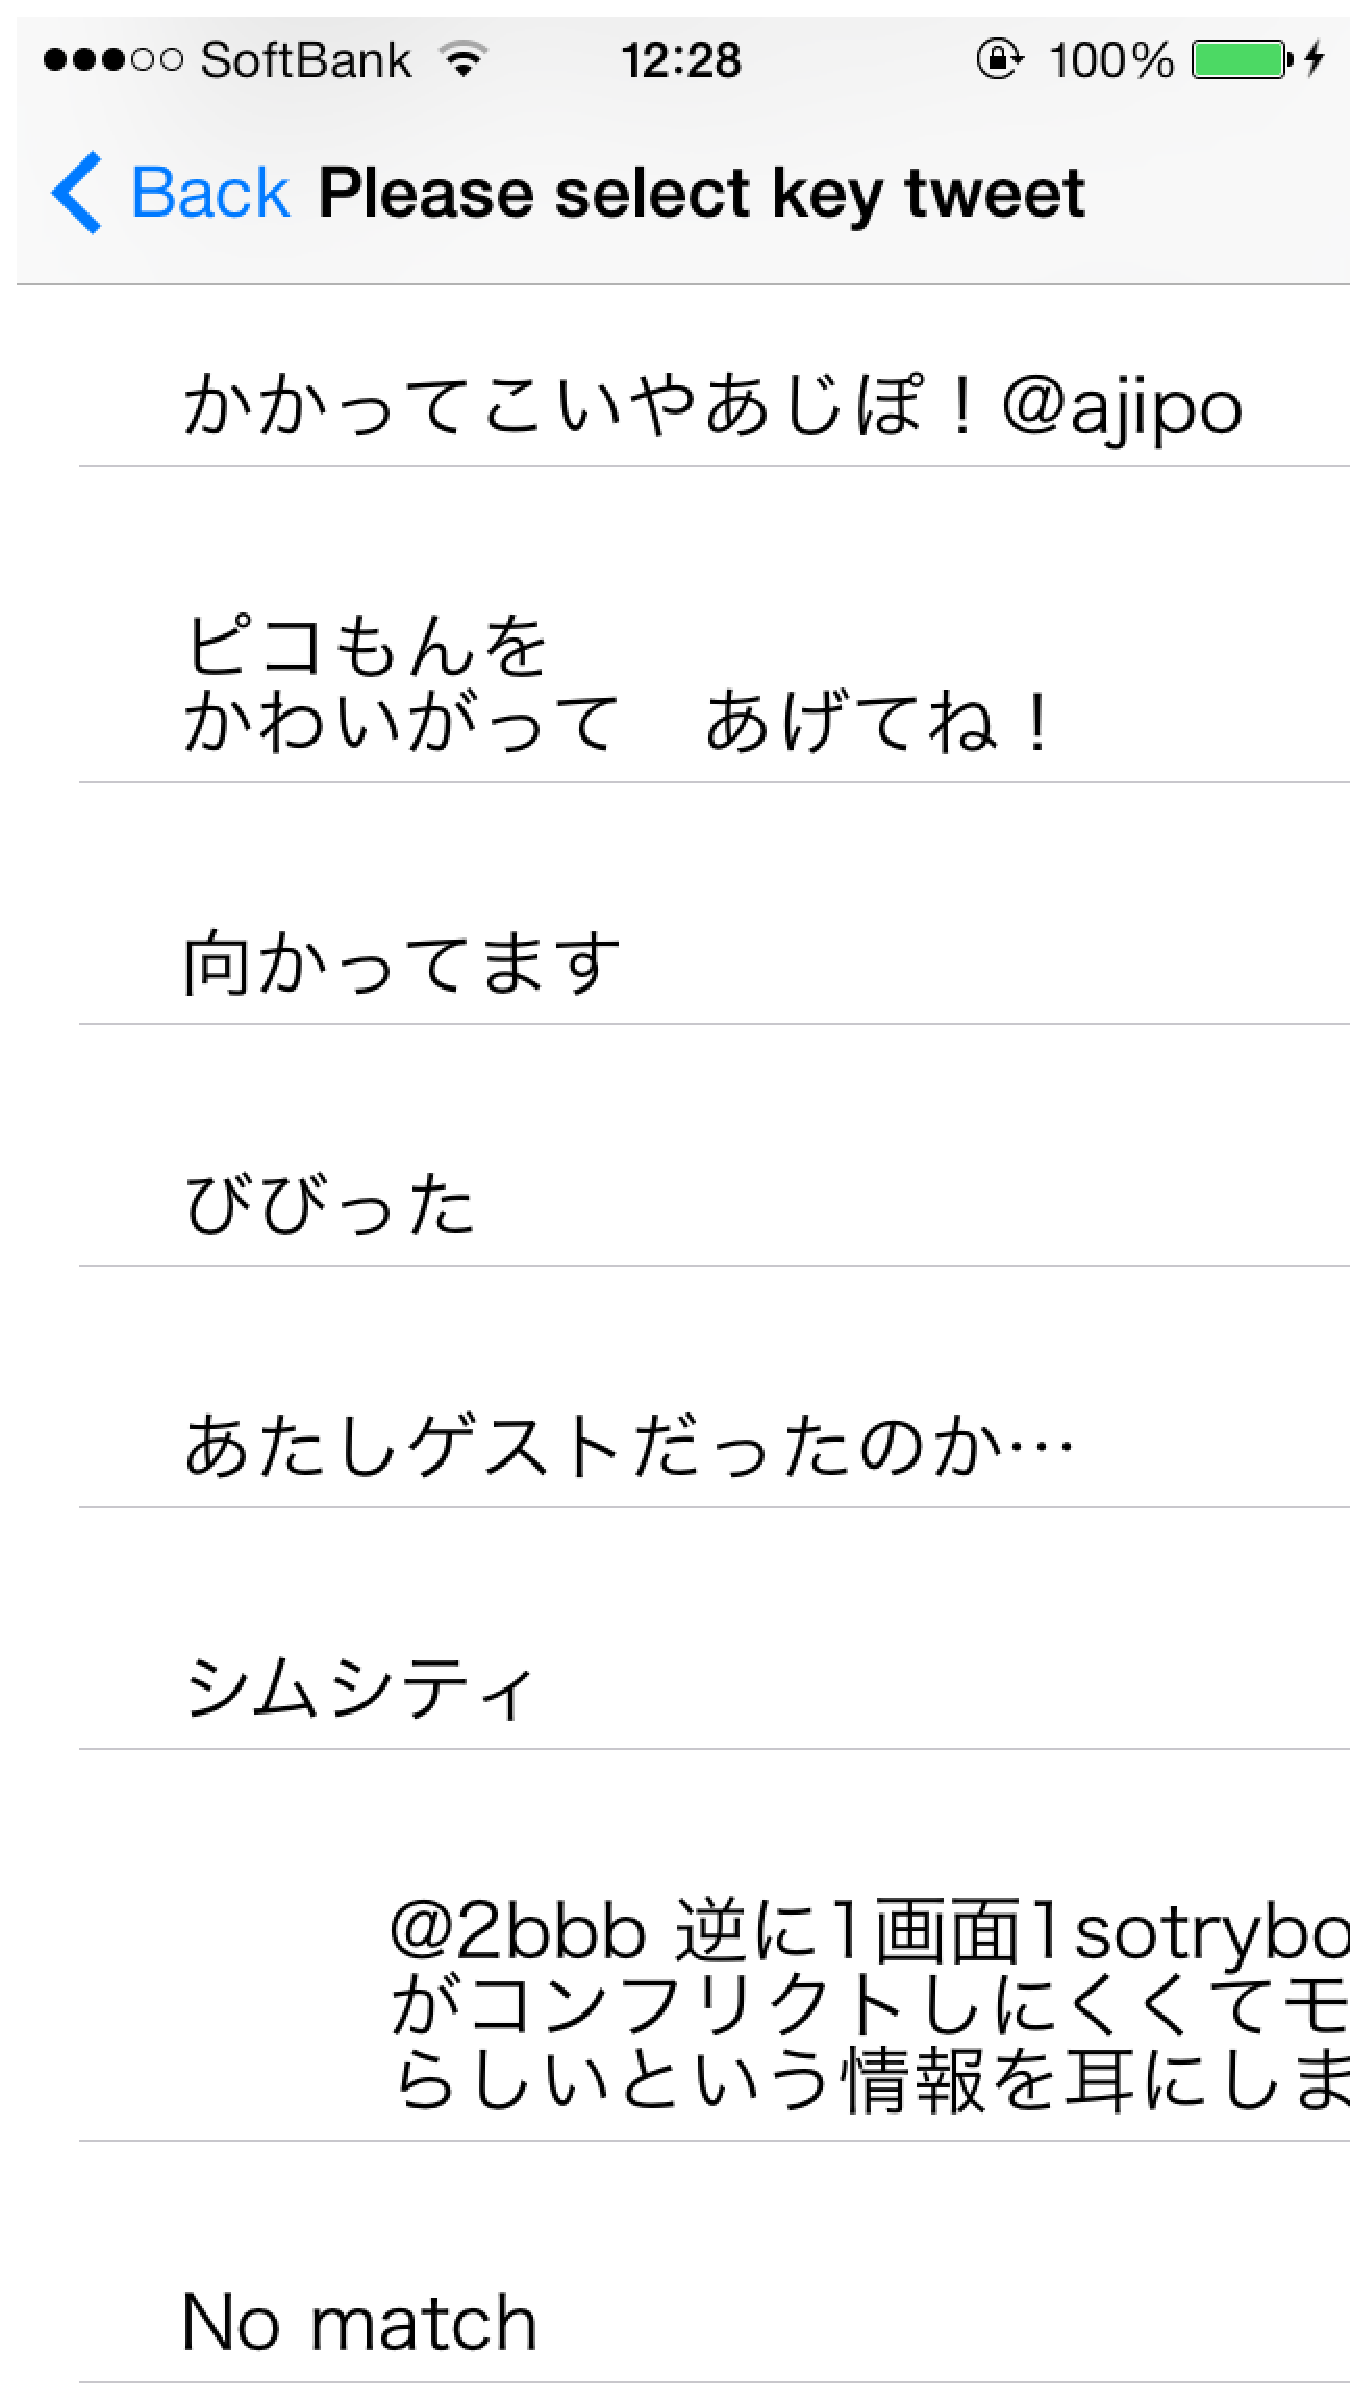
\includegraphics[width=60mm]{img/notifauthNotificationTest.eps}
    \end{center}
    \caption{ロック画面における通知の表示画面を模した認証画面}
    \label{fig:notifauthNotificationTest}
  \end{minipage}
  \begin{minipage}{0.5\hsize}
    \begin{center}
      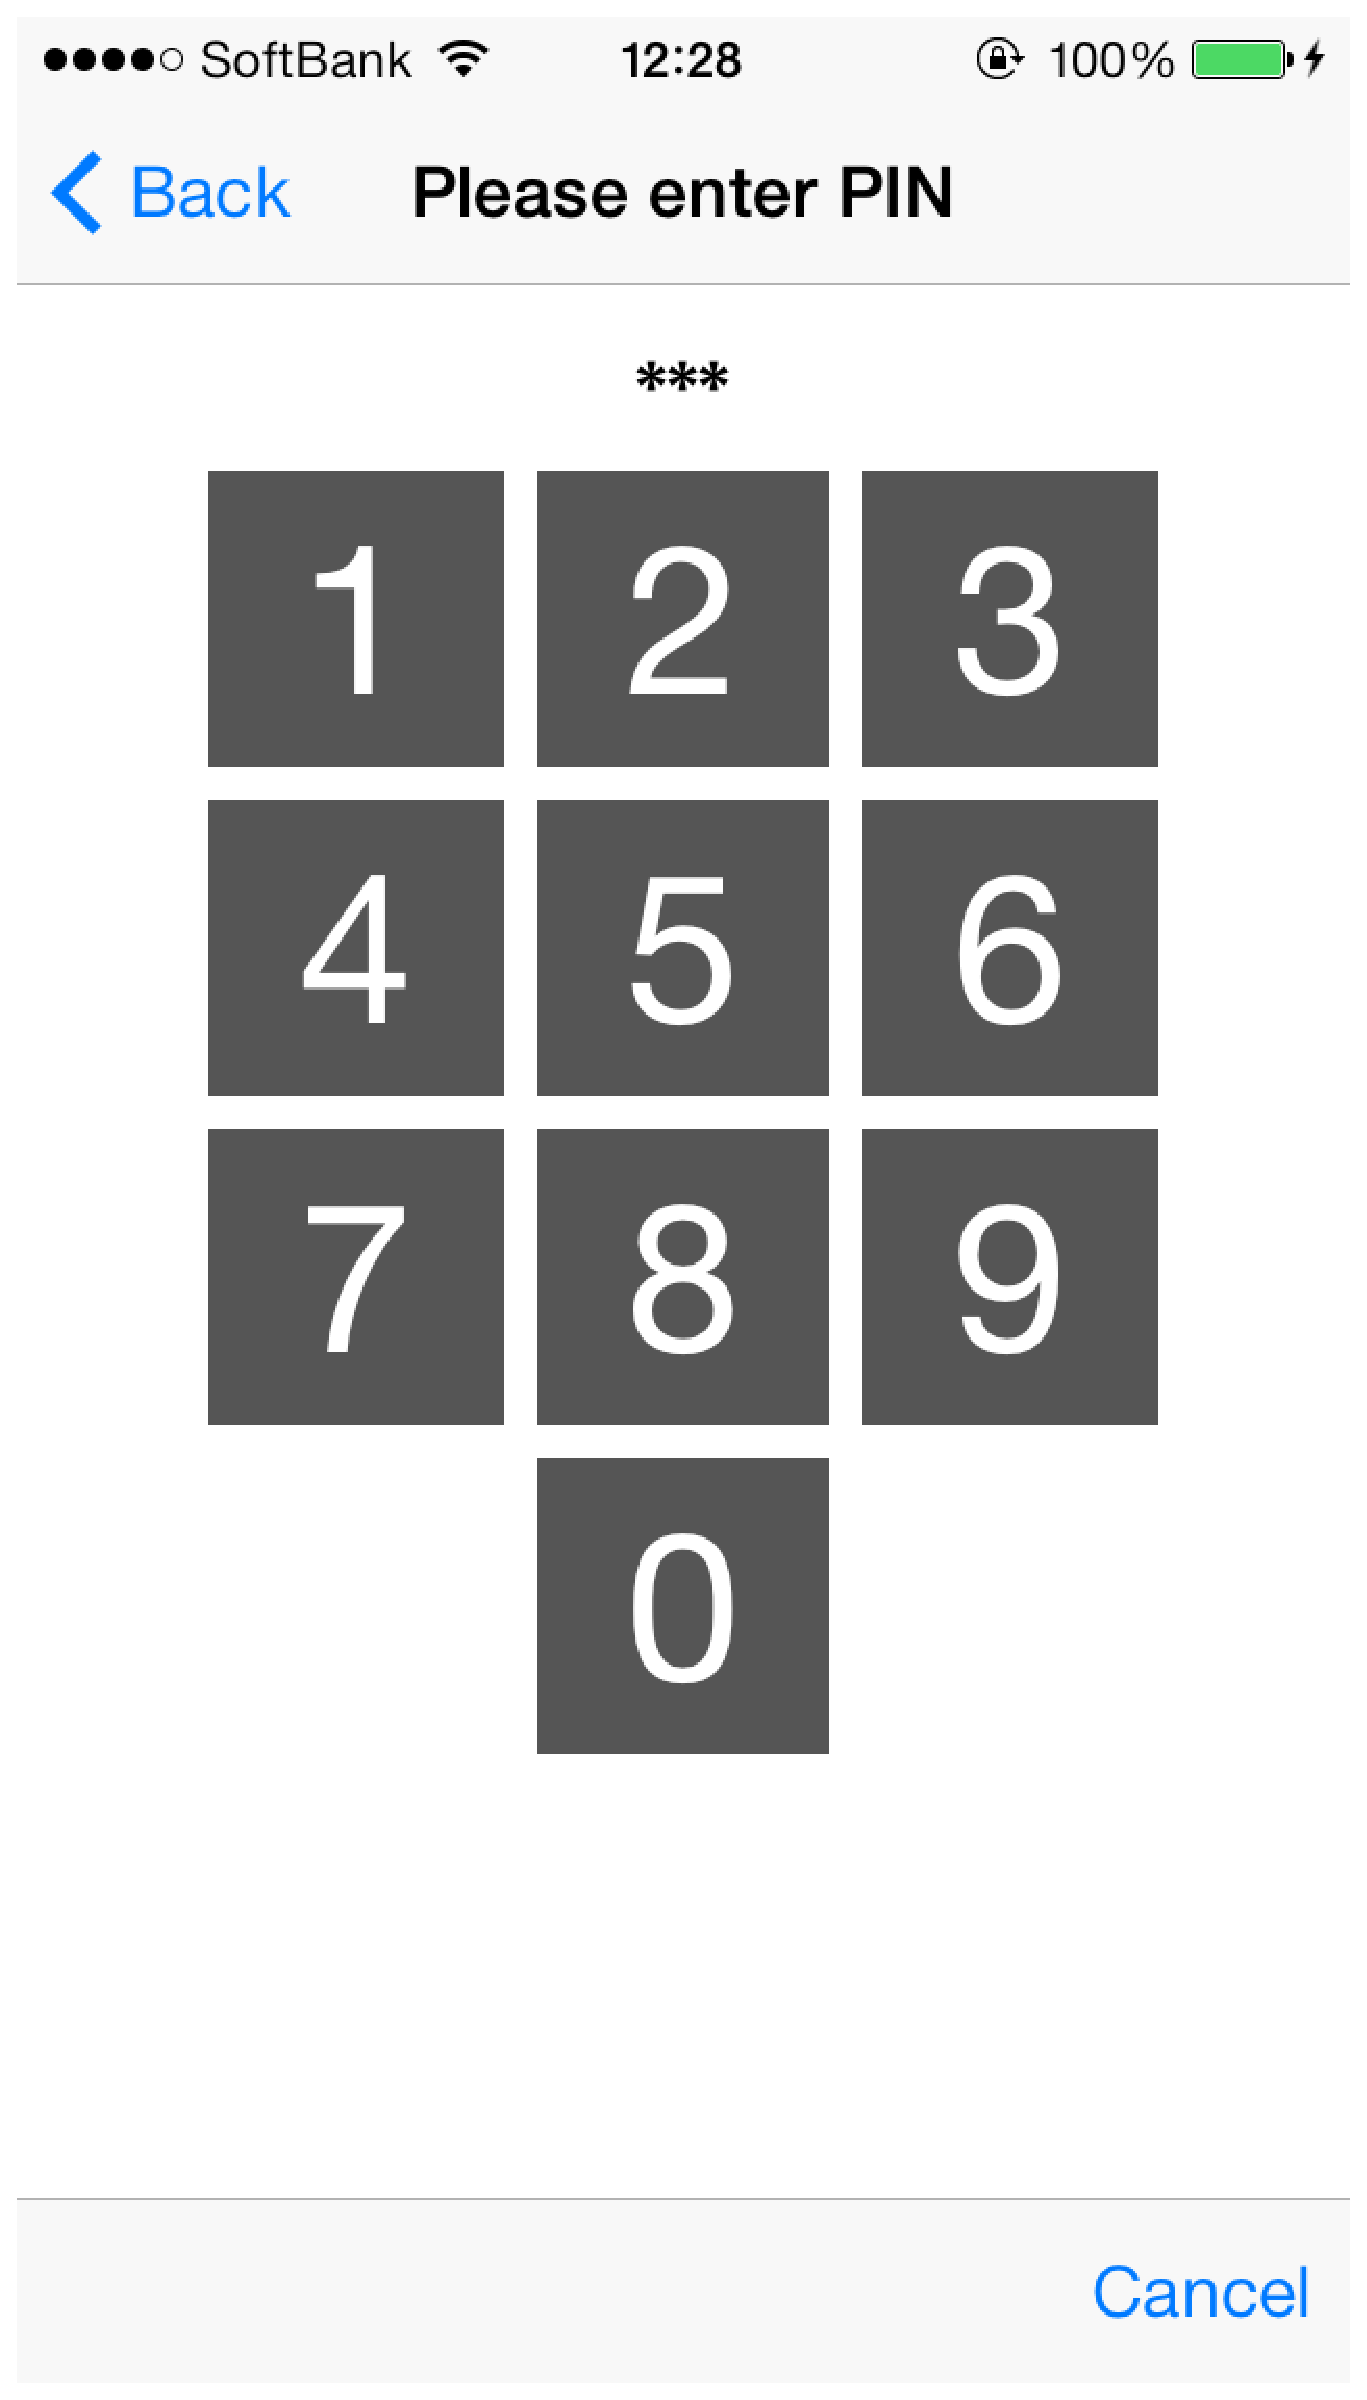
\includegraphics[width=60mm]{img/notifauthPINTest.eps}
    \end{center}
    \caption{ロック画面におけるPINの入力画面を模した認証画面}
    \label{fig:notifauthPINTest}
  \end{minipage}
\end{figure}

\subsection{前提条件}
システムを利用するのに必要な条件や,実装の際に用いた環境などを表\ref{tbl:requirements}に記す.

\begin{table}[htpb]
  \begin{center}
    \caption{必要環境等}
    \label{tbl:requirements}
    \vspace{4mm}
    \begin{tabular}{l||c}
    必要条件 & iOS7を利用し,Twitterアカウントを保持していること \\
    推奨条件 & 定期的に複数のツイートを行っていること \\
    事前準備 & TwitterのOAuthを用いて本ソフトウェアと連携する \\
    実装環境 & Mac OSX 10.9, Xcode5 \\
    動作確認環境 & iPhone 4,iPhone 4S,iPhone 5,iPhone 5S,iPod touch \\
    \end{tabular}
  \end{center}
\end{table}

\section{具体的特徴}\label{sec:feature}
\subsection{時間経過による秘密情報の変化}
Auto Mode Type Termにおいて,設定を行った時から時間が経過すると秘密情報とするツイートが入れ替わる場合がある.
これが成立することの利点としては,
\begin{itemize}
  \item 定期的な秘密情報の変更を能動的に行う必要が低減される
  \item 設定した期間等が秘匿されている限り,出現頻度による攻撃がしにくくなる可能性がある
\end{itemize}
が挙げられる.

また,Auto Mode Type Cycleにおいては,
\begin{itemize}
  \item 新たな秘密情報の候補が出現することで,統計的手法を用いた攻撃に対し強度が高くなる可能性がある
\end{itemize}
ということも利点として考えられる.

欠点としては以下のようなものが挙げられる.
\begin{itemize}
  \item ユーザの本人認証率が下がる可能性がある
  \item 期間の設定やツイートの頻度によっては,ダミーの数が減りすぎることで,統計的手法を用いた攻撃に脆弱になる恐れがある
\end{itemize}

本研究では,以上の利点が本当に作用するかどうかの検証実験も行った.

\newpage

